\begin{figure}[H]
  \centering

  \begin{subfigure}[b]{0.2\textwidth}
    \centering
    
    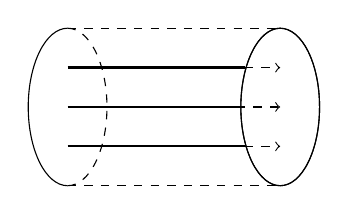
\begin{tikzpicture}
  \draw (0, 1) arc (90 : 270 : 0.5 and 1);
  \draw[dashed] (0, -1) arc (-90 : 90 : 0.5 and 1);

  \draw[thick] (0, -0.5) -- (2.25, -0.5);
  \draw[dashed, ->] (2.25, -0.5) -- (2.7, -0.5);

  \draw[thick] (0, 0) -- (2.15, 0);
  \draw[dashed, ->] (2.15, 0) -- (2.7, 0);

  \draw[thick] (0, 0.5) -- (2.25, 0.5);
  \draw[dashed, ->] (2.25, 0.5) -- (2.7, 0.5);

  \draw (2.7, 0) ellipse (0.5 and 1);
  \draw (2.7, 0) ellipse (0.5 and 1);

  \draw[dashed] (0, 1) -- (2.7, 1);
  \draw[dashed] (0, -1) -- (2.7, -1);
\end{tikzpicture}

    \caption{\(\rot \vec{F} = 0\)}\label{fig:curl}

  \end{subfigure}
  \qquad
  \begin{subfigure}[b]{0.2\textwidth}
    \centering

    \begin{tikzpicture}[
  decoration = {
    markings,
    mark = between positions 0.1 and 1 step 30pt with
      {\arrow[line width = 1pt]{>}}
  }
] 
  \foreach \h in {0, 1, 2} {
    \draw[postaction = { decorate }] (0, \h) ellipse (1 and 0.3);
  };
  \draw[dashed] (-1, 0) -- (-1, 2);
  \draw[dashed] (1, 0) -- (1, 2);
\end{tikzpicture}

    \caption{\(\div \vec{F} = 0\)}\label{fig:solenoidal}

  \end{subfigure}
\end{figure}
